
\subsection{Trouver le meilleur learning rate}
Afin de maximiser nos potentielles performances, nous avons commencé à effectuer un Grid-Search pour trouver le meilleur learning rate possible. Nous avons lancé l'entraînement du LP ResNet sur 5 epochs avec les learning rates suivants : $0.01, 0.005, 0.001, 0.0005, 0.0001$. La Table~\ref{tab:gridsearch} montre alors les résultats de ce Grid-Search. Pour la suite, nous avons pris un learning rate à $0.0005$.

\begin{table}[ht]
    \centering
    \begin{tabular}{cccccc}
    \toprule
    learning rate & acc micro & acc macro & f1-score & top 3 \\
    \midrule
    0.01 & 85.1 & 78.8 & 78.1 & 49.4 \\
    0.005 & 89.1 & 84.7 & 83.6 & \textbf{52.5} \\
    0.001 & 90.4 & 85.7 & 84.8 & 50.5 \\
    0.0005 & \textbf{91.1} & \textbf{86.8} & \textbf{86.0} & 49.1 \\
    0.0001 & 84.9 & 78.6 & 77.4 & 50.4 \\
    \bottomrule
    \end{tabular}
    \caption{Résultat de validation à la fin des entraînements des modèles LP ResNet avec différents learning rate.}
    \label{tab:gridsearch}
\end{table}

\subsection{Entraînement du modèle LP ResNet}
Nous avons entraîné le modèle LP ResNet sur les données de laboratoire sur 10 epochs et un learning rate de $0.0005$. La Figure~\ref{fig: train LP ResNet} montre les courbes d'apprentissage de ce modèle.

\begin{figure}[ht]
    \centering
    \begin{subfigure}{0.32\textwidth}
        \centering
        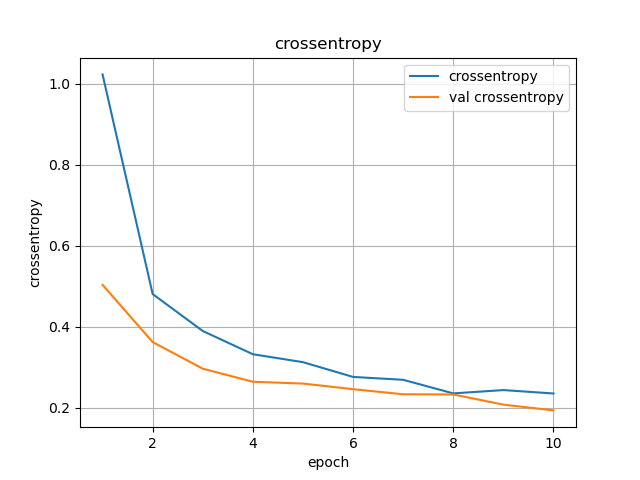
\includegraphics[width=\linewidth]{../logs/resnet_img256_0/crossentropy.png}
        \caption{crossentropy}
    \end{subfigure}
    \begin{subfigure}{0.32\textwidth}
        \centering
        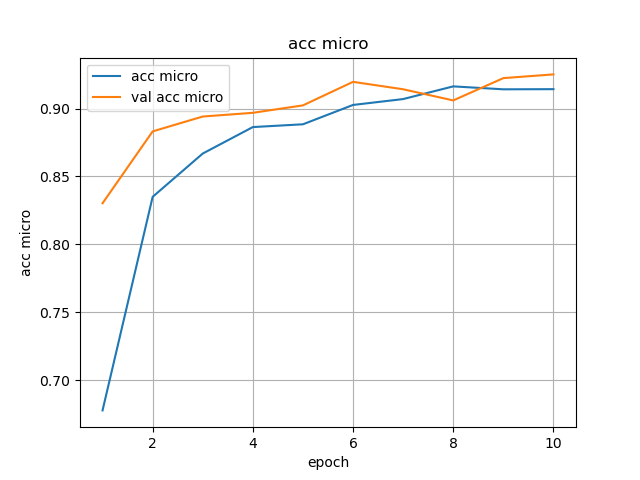
\includegraphics[width=\linewidth]{../logs/resnet_img256_0/acc micro.png}
        \caption{acc micro}
    \end{subfigure}
    \begin{subfigure}{0.32\textwidth}
        \centering
        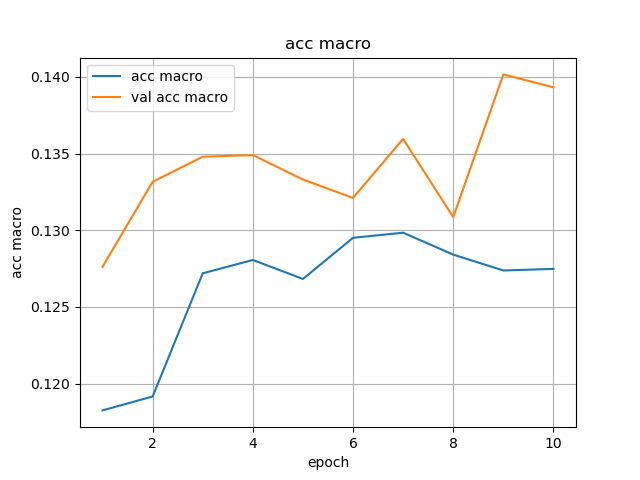
\includegraphics[width=\linewidth]{../logs/resnet_img256_0/acc macro.png}
        \caption{acc macro}
    \end{subfigure}
    \caption{Valeurs de la loss et des accuracy d'entraînement (en bleue) et de validation (en orange) en fonction des epochs durant l'entraînement du modèle LP ResNet.}
    \label{fig: train LP ResNet}
\end{figure}

\subsection{Entraînement du modèle AWL ResNet}
Nous avons entraîné le modèle LP ResNet sur les données de laboratoire sur 20 epochs. Ici, nous avons mis un learning rate de $0.0001$ pour qu'il apprenne moins vite et ne change pas trop ses paramètres dans les couches de convolutions. Nous n'avons pas pu faire une méthode de Grid Search comme le modèle de LP ResNet, en raison du temps d'apprentissage qui est plus long. La Figure~\ref{fig: train AWL ResNet} montre les courbes d'apprentissage de ce modèle.

\begin{figure}[ht]
    \centering
    \begin{subfigure}{0.32\textwidth}
        \centering
        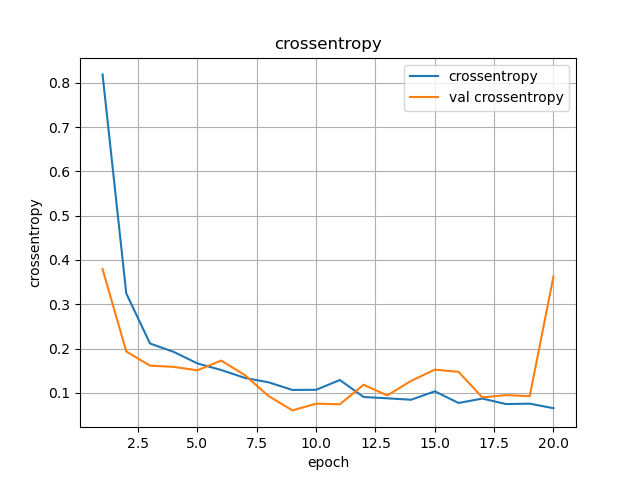
\includegraphics[width=\linewidth]{../logs/resnet_allw_img256_2/crossentropy.png}
        \caption{Crossentropy}
    \end{subfigure}
    \begin{subfigure}{0.32\textwidth}
        \centering
        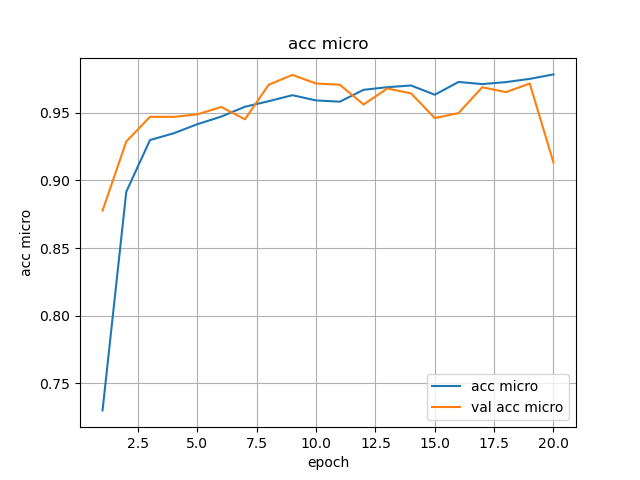
\includegraphics[width=\linewidth]{../logs/resnet_allw_img256_2/acc micro.png}
        \caption{acc micro}
    \end{subfigure}
    \begin{subfigure}{0.32\textwidth}
        \centering
        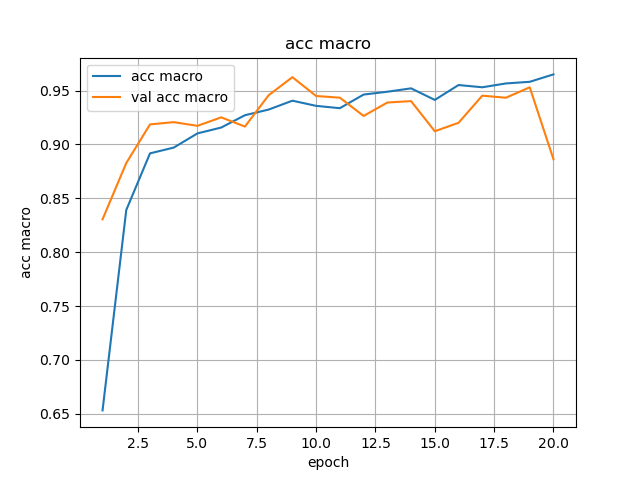
\includegraphics[width=\linewidth]{../logs/resnet_allw_img256_2/acc macro.png}
        \caption{acc macro}
    \end{subfigure}
    \caption{Valeurs de la loss et des accuracy d'entraînement (en bleue) et de validation (en orange) en fonction des epochs durant l'entraînement du modèle AWL ResNet.}
    \label{fig: train AWL ResNet}
\end{figure}

\subsection{Trouver les hyperparamètres pour le modèle Adversarial}
\label{sec: random search}
On cherche ici à trouver le meilleur learning rate pour optimiser le ResNet $lr_{res}$ et pour celui adversarial $lr_{adv}$. On cherche aussi le meilleur paramètre $\alpha$, utilisé dans la formule~\ref{eq: advloss}. On a alors implémenté un Random Search~\cite{randomsearch} et fait 10 expériences de 5 epochs, en prenant à chaque fois des paramètres dans la Table~\ref{tab:random search possibilities}\footnote{On a fait un Random Search et pas un Grid-Search, car il n'est pas possible de tester toutes les combinaisons possibles, qui sont au nombre de 200.}

\begin{table}
    \centering
    \begin{tabular}{cc}
        \toprule
        Paramètres & Valeurs possibles\\
        \midrule
        $lr_{res}$ & 0.01, 0.005, 0.001, 0.005, 0.0001\\
        $lr_{adv}$ & 0.01, 0.005, 0.001, 0.005, 0.0001\\
        $\alpha$ & 0.001, 0.1, 0.5, 1, 2, 5, 10, 100\\
        \bottomrule
    \end{tabular}
    \caption{Liste des valeurs possibles pour les hyperparamètres testés dans le Random Search}
    \label{tab:random search possibilities}
\end{table}

La Table~\ref{tab:random search results} montre les résultats de ce Random Search. \textit{res acc micro} représente l'accuracy micro de la partie ResNet (de même pour \textit{res acc macro}), et \textit{adv acc micro} représente l'accuracy micro de la partie Adversarial. Nous avons donc choisi de prendre les hyperparamètres de l'expérience numéro 2.

\begin{table}[ht]
    \centering
    \begin{tabular}{ccccccc}
    \toprule
    numéro & res acc micro & res acc macro & adv acc micro & $lr_{res}$ & $lr_{adv}$ & $\alpha$ \\
    \midrule
    0 & 79.3 & 72.8 & 82.5 & 0.1 & 1 & 10 \\
    1 & 89.6 & 84.7 & 16.1 & 0.1 & 1 & 0.1 \\
    2 & \textbf{90.8} & \textbf{86.2} & 20.2 & 0.5 & 0.01 & 0.1 \\
    3 & 85.3 & 81.2 & 44.6 & 0.1 & 1 & 0.5 \\
    4 & 88 & 85.7 & 72 & 0.5 & 0.5 & 2 \\
    5 & 89.4 & 85.4 & 56.8 & 0.01 & 0.1 & 0.5 \\
    6 & 89.5 & 85.4 & 71 & 0.1 & 0.1 & 1 \\
    7 & 87.2 & 82.2 & 71.7 & 1 & 0.01 & 1 \\
    8 & 85.3 & 80.3 & \textbf{85.3} & 0.1 & 0.5 & 10 \\
    9 & 86.7 & 83.2 & 84.8 & 0.1 & 0.01 & 10 \\
    \bottomrule
    \end{tabular}
    \caption{Résultat de validation à la fin des entraînements des modèles Adversarial avec différents hypermaramètres.}
    \label{tab:random search results}
\end{table}

\subsection{Entraînement du modèle Adversarial}
Nous avons donc entraîné le modèle Adversarial sur les données de laboratoire sur 20 epochs avec les hyperparamètres trouvés dans la section~\ref{sec: random search}. La Figure~\ref{fig: train adv} montre les courbes d'apprentissages de ce modèle.

\begin{figure}[ht]
    \centering
    \begin{subfigure}{0.32\textwidth}
        \centering
        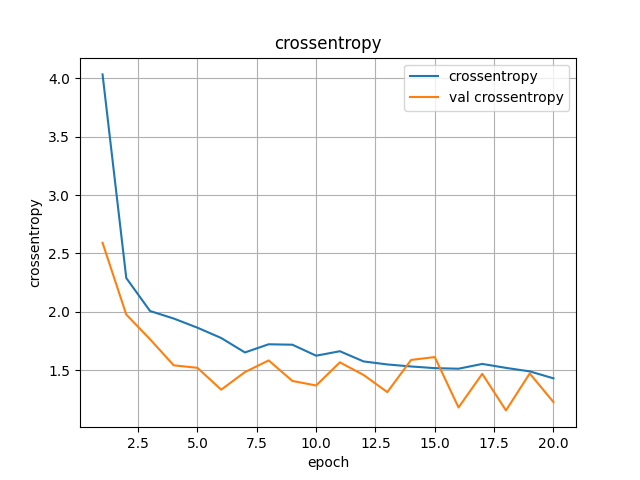
\includegraphics[width=\linewidth]{../logs/adv_img256_1/crossentropy.png}
        \caption{Loss $L_{adv}$}
    \end{subfigure}
    \begin{subfigure}{0.32\textwidth}
        \centering
        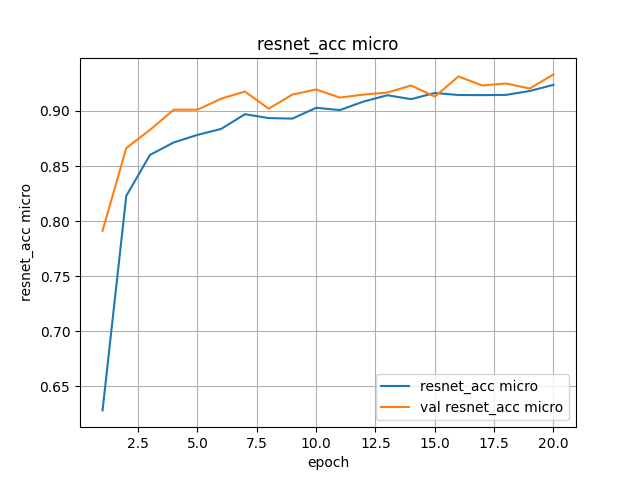
\includegraphics[width=\linewidth]{../logs/adv_img256_1/resnet_acc micro.png}
        \caption{res acc micro}
    \end{subfigure}
    \begin{subfigure}{0.32\textwidth}
        \centering
        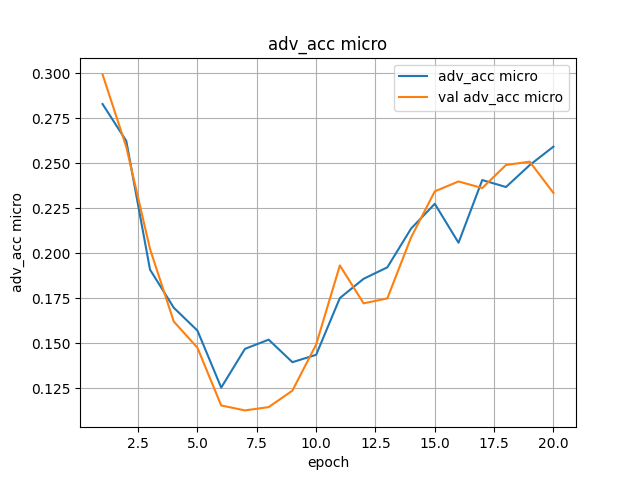
\includegraphics[width=\linewidth]{../logs/adv_img256_1/adv_acc micro.png}
        \caption{adv acc micro}
    \end{subfigure}
    \caption{Valeurs de la loss et des accuracy d'entraînement (en bleue) et de validation (en orange) en fonction des epochs durant l'entraînement du modèle Adversarial.}
    \label{fig: train adv}
\end{figure}

\subsection{Fine-tune des modèles LB ResNet et AWL ResNet}
Nous avons ensuite appris les modèles FT LB ResNet et FT AWL ResNet sur 10 epochs qui sont des modèles fine-tune sur les données réelles à partir des modèles respectivement LB ResNet et AWL ResNet sur 10 epochs. La Figure~\ref{fig: finetune} montre les courbes d'apprentissages de ce modèle.

\begin{figure}[ht]
    \centering
    \begin{subfigure}{0.45\textwidth}
        \centering
        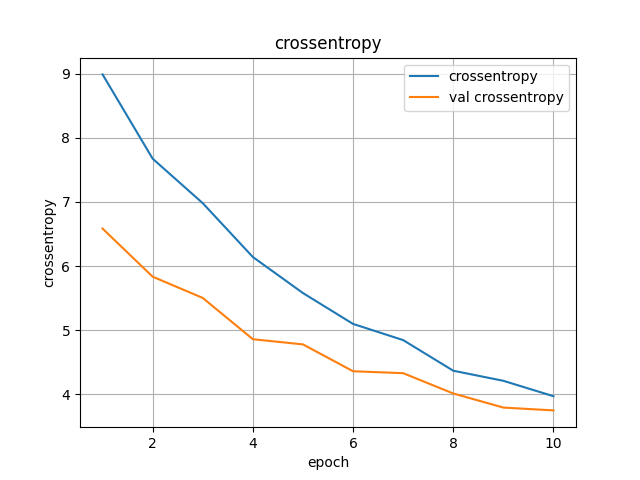
\includegraphics[width=\linewidth]{../logs/retrain_resnet_img256_0/crossentropy.png}
        \caption{crossentropy de FT LP ResNet}
    \end{subfigure}
    \begin{subfigure}{0.45\textwidth}
        \centering
        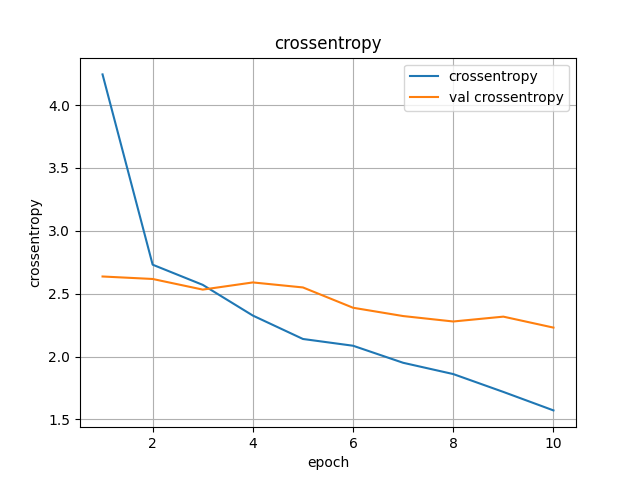
\includegraphics[width=\linewidth]{../logs/retrain_resnet_allw_img256_2/crossentropy.png}
        \caption{crossentropy de FT AWL ResNet}
    \end{subfigure}
    \caption{Valeurs de la loss d'entraînement (en bleue) et de validation (en orange) en fonction des epochs durant l'entraînement des modèles fine-tune sur les données réelles.}
    \label{fig: finetune}
\end{figure}